\documentclass{ecai}
\usepackage{times}
\usepackage{graphicx}
\usepackage{latexsym}
\usepackage{xspace}
\usepackage{hyperref}
\usepackage{algorithm}
\usepackage[noend]{algpseudocode}
\usepackage[numbers]{natbib}
\usepackage{notoccite}
\usepackage{framed}


\usepackage[dvipsnames]{xcolor}
\newcommand{\sergey}[1]{\textcolor{magenta}{{\sc Sergey:} #1}\xspace}
\newcommand{\samuel}[1]{\textcolor{green}{{\sc Samuel:} #1}\xspace}

\newcommand{\constraints}{\ensuremath{\mathcal{C}}\xspace}
\newcommand{\format}[1]{\textit{#1}\xspace}
\newcommand{\generategroups}{\format{generateAssignments}}
\newcommand{\extractgroups}{\format{extractGroups}}
\newcommand{\extracttables}{\format{extractTables}}
\newcommand{\learnconstraints}{\format{learnConstraints}}
\newcommand{\findassignment}{\format{findSolutions}}
\newcommand{\postprocess}{\format{pruneRedundant}}

\newcommand{\CName}{Name\xspace}
\newcommand{\CSignature}{Signature\xspace}
\newcommand{\CFunction}{Function\xspace}
\newcommand{\dependecies}{\ensuremath{\mathcal{D}}\xspace}
\newcommand{\groups}{\ensuremath{\mathcal{G}}\xspace}



%%\ecaisubmission   % inserts page numbers. Use only for submission of paper.
                  % Do NOT use for camera-ready version of paper.

\begin{document}

\title{Tabular Constraint Learning}

\author{Name1 Surname1 \and Name2 Surname2 \and Name3 Surname3 \institute{KU Leuven, Belgium, email: firstname.lastname@kuleuven} }

\maketitle

\begin{abstract}
  abstract
\end{abstract}
\section{Introduction}
\sergey{bullet points for luc to start introduction}\\
\textbf{Key question}:\\
Can we discover or reconstruct structural relations in flat tabular spreadsheet data? [in a general way that allows declarative specification of constraints to discover]\\


\textbf{Motivation}:
\begin{itemize}
  \item File generated from model, model got lost, need to reconstruct
  \item Constraint programming is hard - is Excel hard?
  \item Avoid manual analysis, provide selection of constraints
  \item Error checking
  \item Completion, gain speed and insights (Complicated constraints, also complicated to verify, too much output)
\end{itemize}

\textbf{Novelty:}
\begin{itemize}
  \item Unsupervised setting (contrary to flashfill, etc)
  \item Numeric, different constraints (contrary to single textual function solution in flashfill, etc)
  \item Data format (2D) -- data is no longer in rows like a classic ML or DM settings
  \item Declarative, general / modular, stacking of constraint problems 
\end{itemize}

\sergey{need to elaborate the example here: like in a story} 

\begin{figure*}[tbh]
  \begin{center}
    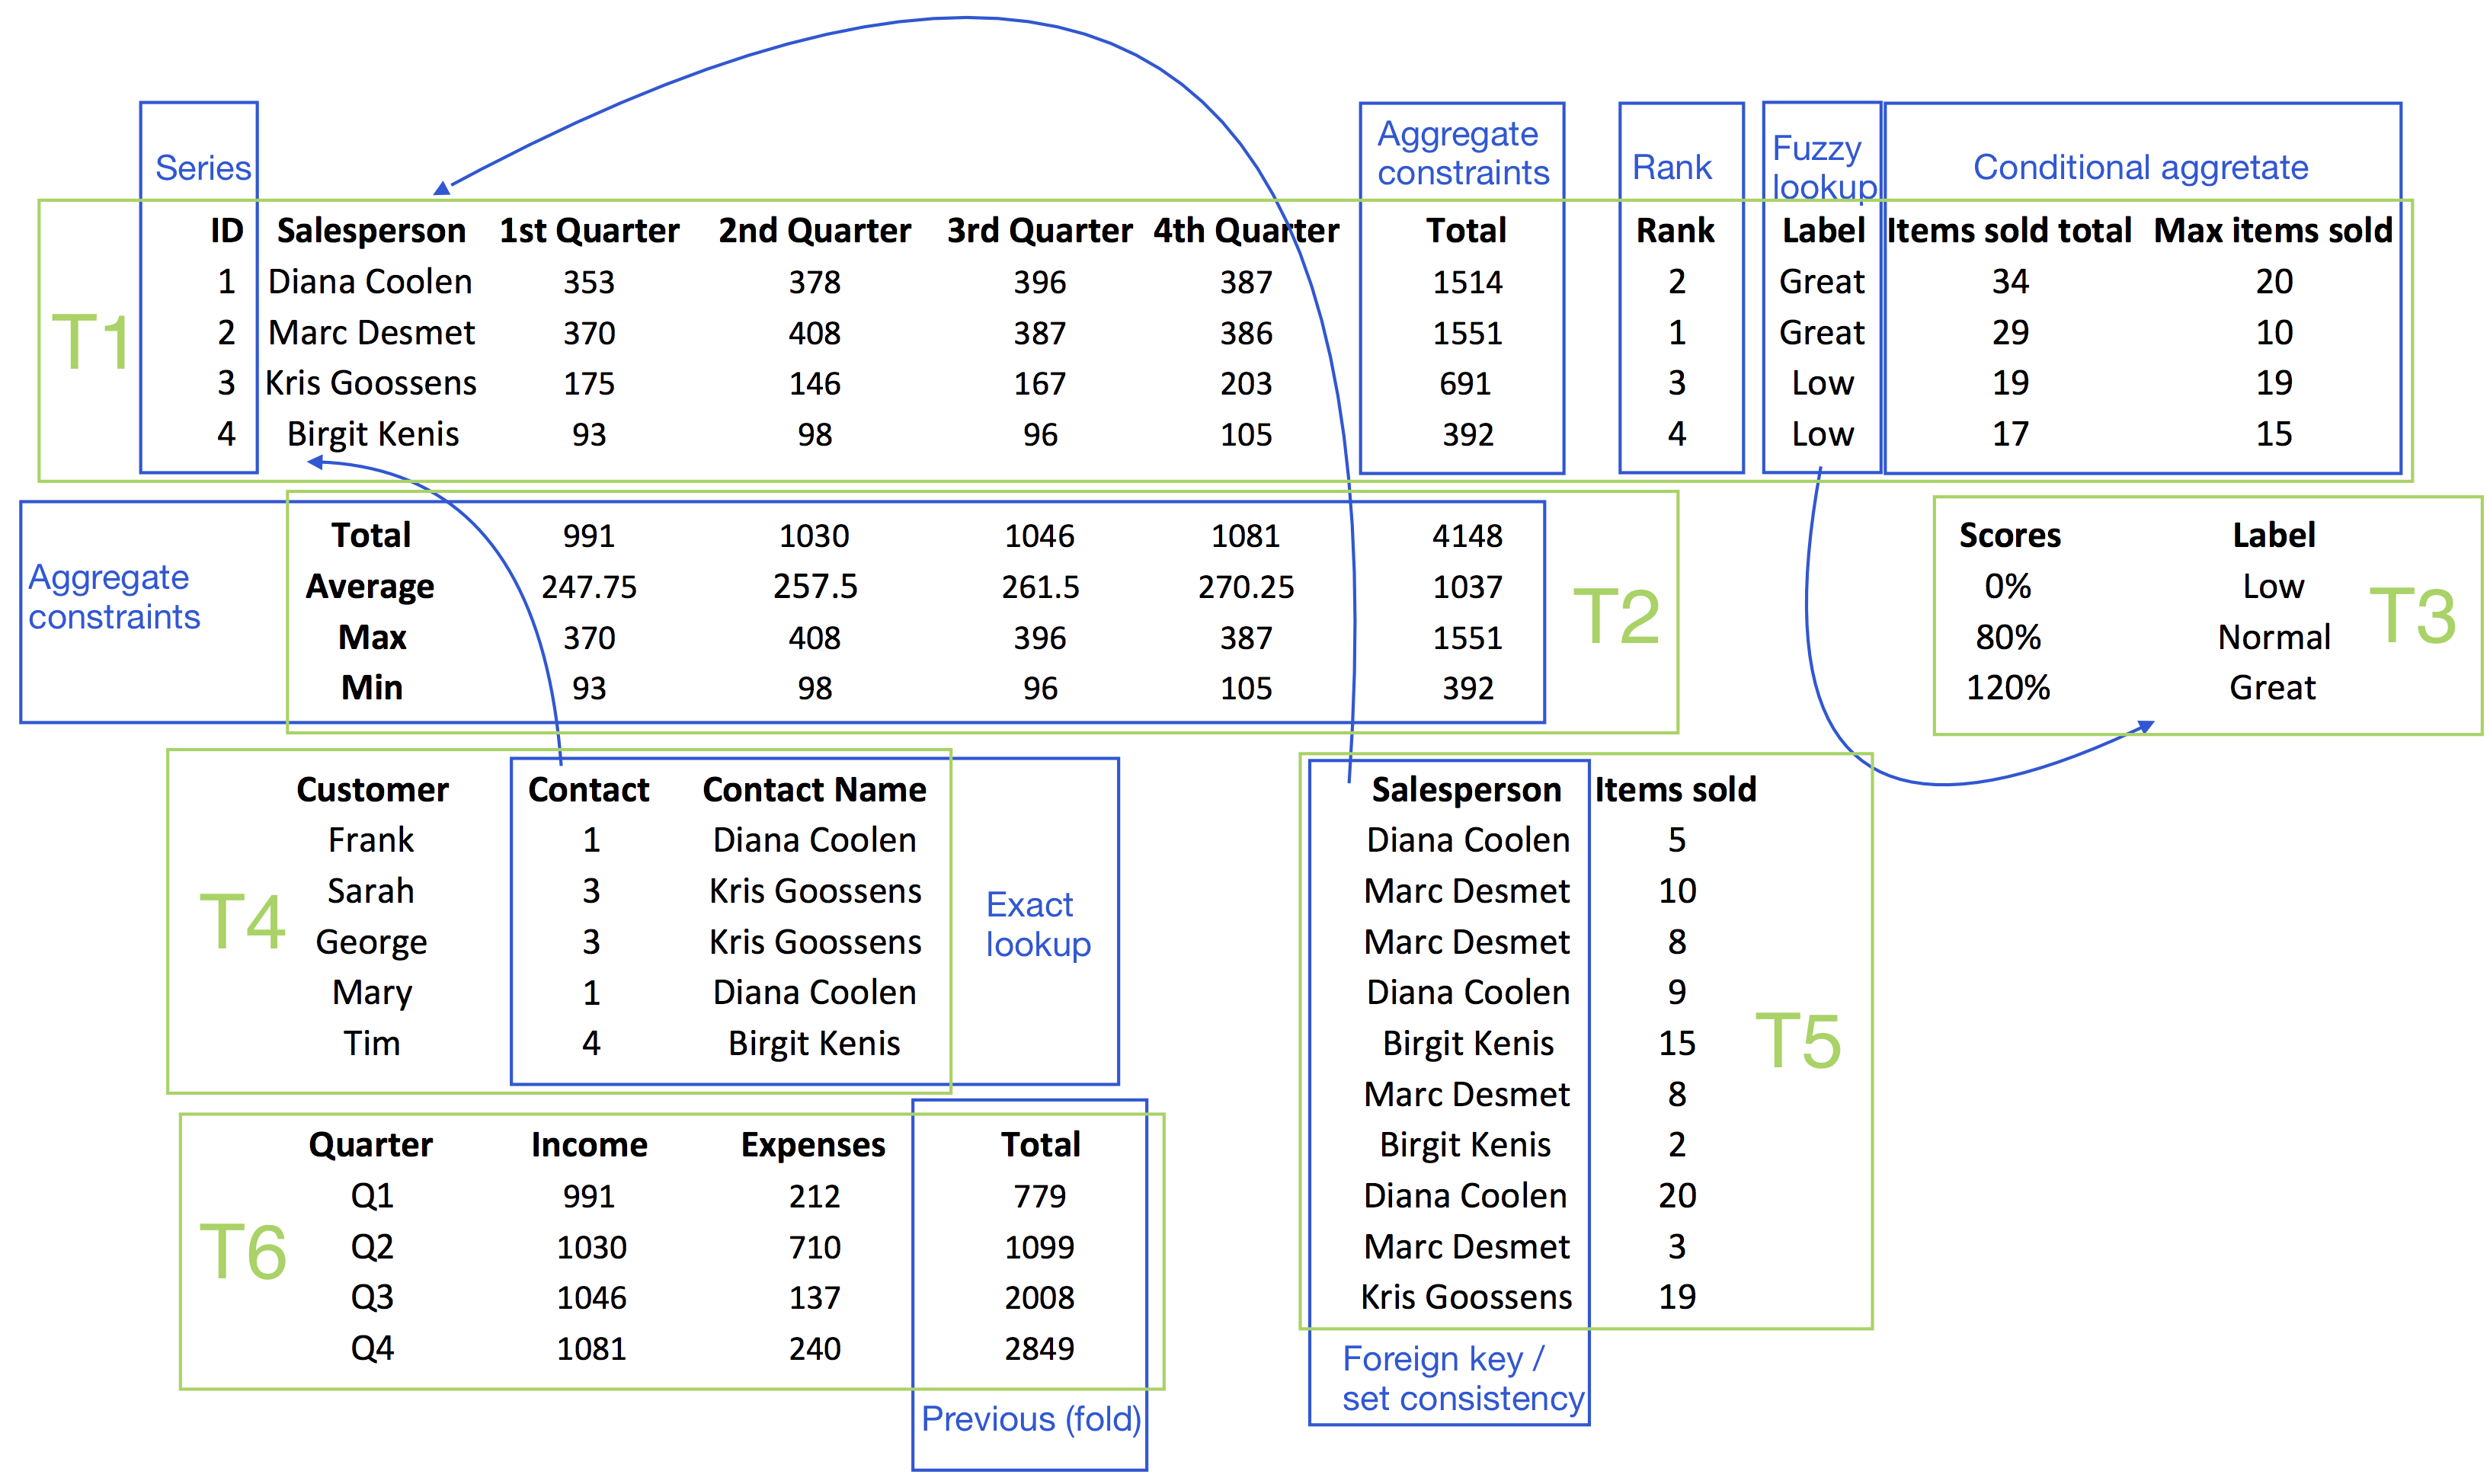
\includegraphics[width=0.75\textwidth]{figures/Demo.png}
  \end{center}
  \vspace{-10pt}
  \caption{An example of constraint reconstruction (in blue) with indicated groups (in green)}
  \label{fig:main_example}
\end{figure*}

\section{Formalization}


\begin{algorithm}[thb]
  \begin{algorithmic}
    \footnotesize
    \State \textbf{Input:} $G$ -- set of groups
    \State \textbf{Output:} $S$ -- learned constraints with their satisfaction assignments
    \State $S \gets \emptyset$ \Comment{The set of solutions}
  \For{$c \in \constraints$} \Comment{\constraints -- partially ordered set of Excel constraints; Table \ref{table:constraints}}
  \State $v_1, ..., v_n =$ variables of $c$ 
    \For{$v_1{:}~G_1, \dots, v_n{:}~G_n \in \generategroups(c, G, S)$}
      \State $S \gets S \cup \findassignment(c, v_1{:}~G_1, \dots, v_n{:}~G_n, S)$
    \EndFor
  \EndFor\\
\Return $S$
\end{algorithmic}
\caption{Tabular constraint learning}
\label{algo:tcl}
\end{algorithm}
\subsection{Groups, Type-consistency and Constraints}
In this work we distinguish the following types of data: numeric and textual. The numeric type has two subtypes: integers and floats. We also consider the special element called \textit{None}, which has two types: numeric and textual. A set is called \textit{type-consistent} iff all elements are either numeric or textual. Certain constraints, such as \textit{rank} or \textit{series}, make use of the numeric sub-types by requiring its arguments to be integers.

A \textit{vector} is either a column or a row that is type-consistent. If a vector is a row (column), we say that it has a \textit{row} (\textit{column}) orientation. A \textit{group} is a subrange of vectors with the same orientation in a table. We use the following notation to refer to a row (column) group $G$ in a table $T$ with rows (columns) ranging from $a$ to $b$: $G = T[a{:}b,:]$ ($G = T[{:},a{:}b]$), where $a,b$ are natural numbers. We denote as the \textit{length} of a row (column) group $G$, written as \textit{length(G)}, the number of its columns (rows). We call a group $G$ \textit{numeric} (\textit{textual}, etc), written as \textit{numeric(G)}, if its vectors contain numeric (textual, etc) elements.

An \textit{Excel constraint} is a triple \textit{(\CName, \CSignature, \CFunction)}. Let us elaborate on each of them. \textit{\CName} is the textual name of the constraint together with its variable names. \textit{\CSignature} is a set of constraints specifying the properties of the group assignments, corresponding to the variables in \CName, such as their types, e.g., requiring them to be integers or constraining the sizes, e.g. the length of vectors in the arguments must be equal. These are constraints on the group meta-information not on the actual group content. \textit{\CFunction} is a set of constraints specifying that the data in the subgroups satisfies the function. For example, an excel constraint \textit{rank} has \CName \textit{Y = RANK(X)}, where $X$ and $Y$ are the variables; its \CSignature is: the group $G_X$ (associated with X) is numeric, $G_Y$ is integer and the length of vectors in $G_X$ is the same as in $G_Y$; its \CFunction is the following constraint: a pair of vectors $X,Y$ is a solution iff $X \in G_X, Y \in G_Y$ and each value in $X$ has the rank (possibly with ties) specified in $Y$.

\section{Problem Statement}
In the previous section we introduced the problem of tabular constraint learning informally using the example in Figure \ref{fig:main_example}. Here we formalize the statement in terms of Excel constraints and group assignments.

\begin{framed}
  \begin{tabular}{ll}
  
    \multicolumn{2}{c}{{\textbf{Tabular Constraint Learning Problem}}}\\
    &\\
    \textbf{Given:} & The set of all groups $\groups$ and the set of Excel  \\
    \phantom{Given:} & constraints $\constraints$ with its dependencies DAG $\dependecies$\\
    \textbf{Find:} & For each constraint $c$ in \constraints all the subgroups of $\groups$ satisfying the \CSignature and \CFunction of $c$
  \end{tabular}
\end{framed}

\section{Approach to Tabular Constraint Learning}
Let us describe the key steps and functions in Algorithm \ref{algo:tcl}. Essentially, the algorithm has two steps: candidate group generation and subgroup satisfaction search, which is in line with the ``generate-and-test'' paradigm that is well-known in AI \cite{whaisasp}. Let us elaborate on each step in detail.

\paragraph{Candidate group generation} $\generategroups(\textit{Constraint,GroupSet,Solutions})$ is the function generating tuples of groups that are legitimate solution candidates e.g., $X,Y$ are variables of \textit{Y = RANK(X)} and $X,Y$ satisfy the constraints from \CSignature above. Essentially, the group generation step is a constraint satisfaction problem associated with the specific constraint. However, many constraints have the same candidate generation procedures, e.g., sum, min, max, avg, count, etc.

\paragraph{Subgroup satisfaction search} $\findassignment(\textit{Constraint,Candidates,Solutions})$ is the function looking for the subsets of vectors in the candidates satisfying the constraint. If multiple subsets satisfy the constraint, a maximal is selected. If $G_1,G_2$, associated with the variables $X,Y$ in the constraint \textit{Y = RANK(X)}, are candidates, then \findassignment selects a single vector $y$ in $G_2$ and a single vector $x$ in $G_1$ such that $x$ is ranked by $y$. For example, in Figure \ref{fig:main_example} the group $G = T_1[{:},3{:}8]$ serves as $X$ and $Y$ and $x$ can be picked as $T_1[{:},7]$ and $y$ would be $T_1[{:},8]$.

\subsection{Constraints}
The set of Excel constraints has a partial order in which they should be learned. For certain constraints this order does not matter, such as rank or product. For many others they have to be learned in the order, which is specified as a DAG in Figure \ref{fig:learning_order} (if a constraint is not in the graph, it is independent). This figure specifies a potential parallelization of the computation, since each connected component is independent of the others.

\begin{figure}[htb]
  \centering
  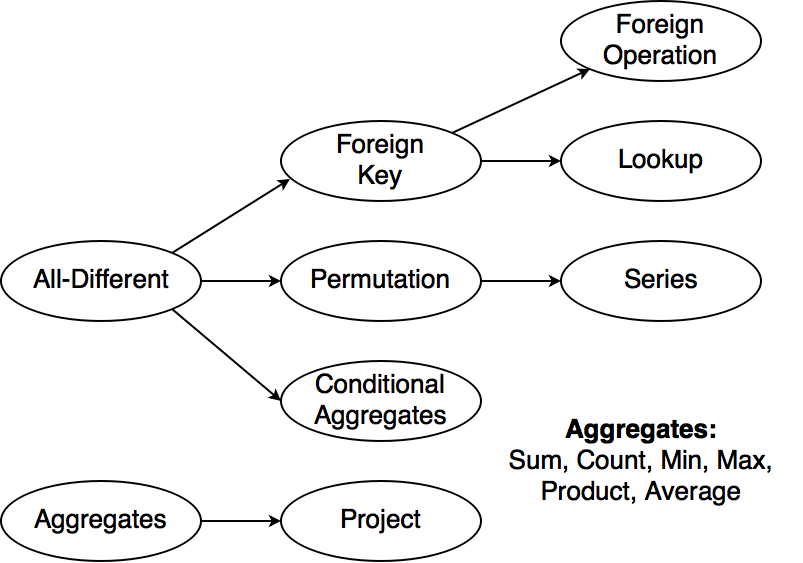
\includegraphics[width=0.20\textwidth]{figures/constraint_dependency.png}
  \caption{Constraint Learning Order. The \textcolor{green}{solid} arrows indicate a construction order, i.e., learning one constraint is necessary to build the other. The \textcolor{red}{dashed} arrows indicate a pruning order, the former constraint is used to prune the latter.}
  \label{fig:learning_order}
\end{figure}


\newcommand{\numeric}{\format{numeric}}
\newcommand{\textual}{\format{textual}}
\newcommand{\integer}{\format{integer}}
\newcommand{\length}{\format{length}}
\newcommand{\nat}{\mathcal{N}}

\begin{table*}
  \centering
  \begin{tabular}{ccc}
    \textbf{\CName} & \textbf{\CSignature} & \textbf{\CFunction}\\
    ALLDIFFERENT(X) & $\textual(G_X) \vee \integer(G_X) $ & $X \in G_X{:}~\forall i,j \in \nat{:}~i \neq j \rightarrow X[i] \neq X[j]$ \\
    X = Y & & \\
    FK -> PK & & \\
    R = PRODUCT(FV, FK=PK | PV) & & \\
    FV = FUZZY-LOOKUP(FK, PK, PV) & & \\
    FV = LOOKUP(FK, PK, PV) & & \\
    PERMUTATION(X) & & \\
    R = O1 * O2 & & \\
    R = PROJECT(P) & & \\
     Y = RANK(X)     & $\numeric(G_X) \wedge \integer(G_Y) \wedge \length(G_X) = \length(G_Y)$ & $\begin{array}{r} X \in G_X, Y \in G_Y{:}~\forall i,j \in \nat{:}~(Y_i \leq Y_j \rightarrow X_{Y_i} \leq X_{Y_j}) \\ \wedge~ 1 \leq Y_i \leq \length(G_Y) \end{array}$ \\
    A = PREV(A) + P - N & & \\
    SERIES(X) & & \\
    Y = SUM(X, col) & & \\
    Y = SUM(X, row) & & \\
    R = SUMIF(FK=PK, V) & & \\
    R = SUMPRODUCT(O1, O2) & & \\

  \end{tabular}
  \caption{Excel Tabular Constraints \sergey{Luc, we need your comments here on the notation of $X,Y$ and $G_X,G_Y$}}
  \label{table:constraints}
\end{table*}

\subsection{Workflow}
\begin{algorithm}[thb]
  \begin{algorithmic}
    \footnotesize
    \State \textbf{Input:} $D$ -- dataset, (optional: tables $T$, groups $G$)
    \State \textbf{Output:} $S$ -- learned constraints with their satisfaction assignment
    \If{$T$ is \textbf{not} provided}
      \State $T \gets \extracttables(D)$
    \EndIf
    \If{$G$ is \textbf{not} provided}
      \State $G \gets \extractgroups(D, T)$
    \EndIf
    \State $S \gets \learnconstraints(G)$
    \State $S \gets \postprocess(S)$
    \State \Return $S$
\end{algorithmic}
\caption{Workflow}
\label{algo:workflow}
\end{algorithm}

\section{Case Study aka Experiments}

\textbf{Approach}
\begin{itemize}
  \item Notation
  \item Algorithm (select constraints, find assignments, find solutions)
\end{itemize}

{\bfseries 
  Experimental questions
}
\begin{itemize}
  \item  How accurate are we? (Accuracy / recall)
  \item  How fast are we and which factors affect the runtime (how)?
  \item  How general is our approach, what limitations are there?
\end{itemize}


\section{Related Work}
\sergey{key bullet points for Luc and possibly Samuel and me to make related work section}

\sergey{ECAI reference style file ignores their guideline and their guideline ignores what is written in the guidelines!}
flashfill, flashextract, flashmeta \cite{flashfill,flashextract,flashmeta}
\begin{itemize}
  \item their supervised vs our unsupervised approach
  \item they look for a single ``smallest'' solution, we enumerate them all
  \item they are looking for a function, we solve constraint satisfaction problems
  \item we do not assume classic row based data layout, we work in the tabular setting
\end{itemize}

sketch \cite{sketch}
\begin{itemize}
  \item look for a constant that would fill in the gap in a program
  \item tailored for programming languages
  \item similar to model checking
  \item looks for a single solution
  \item similar to constraint satisfaction and sat, where one is interested in a single assignment that works for any potential input
\end{itemize}

tabular \cite{tabular}
\begin{itemize}
  \item language based on the excel tables that specify probabilistic models
  \item a system for probabilistic inference and similarity mostly in the usage of excel
  \item probabilistic constraint satisfaction (?) and graphical models
  \item single solution again
\end{itemize}

modelseeker \cite{modelseeker} \sergey{Samuel, Luc, probably you would need elaborate here more in details}

\begin{itemize}
  \item not designed for excel-like data representation (type consistency, groups, etc)
  \item not designed for excel-like constraints (lookups, conditional ifs, etc)
  \item does not support user extensions (?)
\end{itemize}

claudien \cite{claudien} \sergey{Samuel, Luc, you would need to help with this one}

\bibliographystyle{ecai}
\bibliography{references}
\end{document}
%%%%%%%%%%%%%%%%%%%%%%%%%%%%%%%%%%%%%%%%%%%%%%%%%%%%%%%%%%%%%%%%%%%%%%
